%=========================================================================
% (c) Michal Bidlo, Bohuslav Křena, 2008

\chapter{Introduction}
The C programming language is a very powerful and effective way of writing programs. Arguably the most important reason is that it is almost as low-level as a structured programming language can be. This leads to great freedom of choice and potentially very effective resulting program, however with this freedom comes a programmer's responsibility to either evade some language constructs or to cope with possible unpredictable results -- the undefined behavior in C.

The most important document to study regarding the C language is its most recent standard: ISO/IEC 9899:2011~\cite{C11} , informally known as \emph{ISO C11}. (For the purpose of this paper, I am going to cite its last free and public draft available~\cite{WG14N1570})

%%%%%%%%%%%%
\section{Undefined behavior}
ISO C11 specifies how the implementation is expected to work and when there are no expectations regarding the implementation's behavior at all. Multiple terms are used to describe similar but different requirements on the implementation:~\cite{WG14N1570}
\begin{itemize}
    \item \emph{Behavior} -- external  appearance or action
    \item \emph{Unspecified behavior} -- use of an unspecified value, or other behavior where this International Standard provides two or more possibilities and imposes no further requirements on which is chosen in any instance
    \item \emph{Implementation-defined behavior} -- unspecified behavior where each implementation documents how the choice is made
    \item \emph{Locale-specific behavior} -- behavior that depends on local conventions of nationality, culture, and language that each implementation documents
    \item \emph{Undefined behavior} -- behavior, upon use of a nonportable or erroneous program construct or of erroneous data, for which this International Standard imposes no requirements
\end{itemize}

Bear in mind that undefined behavior allows \emph{any} behavior -- meaning not only the returned value is not specified but also that the implementation is allowed to do \emph{anything} -- the program might run ``just fine'' (as the programmer expected) or the program might erase your hard disk and it would be perfectly legal according to the standard.

%%%%%%%%%%%%
\section{Side effect}
ISO C11~\cite{WG14N1570} gives the following definition for a side effect: ``Accessing a volatile object, modifying an object, modifying a file, or calling a function that does any of those operations are all side effects, which are changes in the state of the execution environment. Evaluation of an expression in general includes both value computations and initiation of side effects. Value computation for an lvalue expression includes determining the identity of the designated object.''

Informally said, a side effect is usually modifying a memory during evaluation of an expression -- for example \verb|i++| is an expression whose \emph{return value} is the value of \verb|i| before evaluation \emph{and the value of }\verb|i|\emph{ is incremented by 1} -- this is the side effect, the expression evaluation accesed the memory addressed by \verb|i| and modified its value.

%%%%%%%%%%%%
\section{Sequence point}
The C standard~\cite{WG14N1570} states that ``Sequenced before is an asymmetric, transitive, pair-wise relation between evaluations
executed by a single thread, which induces a partial order among those evaluations.
Given any two evaluations A and B, if A is sequenced before B, then the execution of A
shall precede the execution of B. (Conversely, if A is sequenced before B, then B is
sequenced after A.) If A is not sequenced before or after B, then A and B are
unsequenced. Evaluations A and B are indeterminately sequenced when A is sequenced
either before or after B, but it is unspecified which. The presence of a sequence point
 between the evaluation of expressions A and B implies that every value computation and
side effect associated with A is sequenced before every value computation and side effect
associated with B.''

This means that the evaluation order of expressions may and may not be specified and if it is not, the implementation may and may not be required to specify it and do it consistently and predictably. ISO C11, in other words, states that an expression A must be evaluated (or at least the external behavior must appear like it is evaluated -- ``an actual implementation need not evaluate part of an expression if it can deduce that its value is not used and that no needed side effects are produced''~\cite{WG14N1570}) before an expression B when it is on the left side of a sequence point that is between A and B. Otherwise A and B may either be evaluated in an unspecified order or they can even \emph{not be evaluated in any order} -- the evaluation of A may start, then be interrupted, B may be evaluated and A evaluation may be completed then, for example.

ISO C11 enumerates the sequence points as follows:~\cite{WG14N1570}
\begin{itemize}
    \item Between the evaluations of the function designator and actual arguments in a function call and the actual call.
    \item Between the evaluations of the first and second operands of the following operators: logical AND $\&\&$ ; logical OR $\|$ ; comma , .
    \item Between the evaluations of the first operand of the conditional ? : operator and whichever of the second and third operands is evaluated.
    \item The end of a full declarator
    \item Between the evaluation of a full expression and the next full expression to be evaluated. The following are full expressions: an initializer that is not part of a compound literal; the expression in an expression statement; the
controlling expression of a selection statement (if or switch); the controlling expression of a while or do statement; each of the (optional) expressions of a for statement; the (optional) expression in a return statement.
    \item Immediately before a library function returns.
    \item After the actions associated with each formatted input/output function conversion specifier.
    \item Immediately before and immediately after each call to a comparison function, and also between any call to a comparison function and any movement of the objects passed as arguments to that call.
\end{itemize}

%%%%%%%%%%%%
\section{Consequences}%FIXME: str. 76 normy, body 2 a 3, zminit. That means whenever there are two expressions that are unsequenced and have multiple side effects OR a side effect and an access on the same object...
According to ISO C11~\cite{WG14N1570}, undefined behavior occurs when ``a side effect on a scalar object is unsequenced relative to either a different side effect on the same scalar object or a value computation using the value of the same scalar object''. That means whenever there are two expressions that are unsequenced and have a side effect on the same object (meaning its value is to be modified, but in any order and possibly not even in any order), the undefined behavior occurs meaning not only the value of a given object is undefined but the whole program might do absolutely anything -- most of the implementations will probably do something ``reasonable'', but they are not required to.

This kind of undefined behavior appears not to be very dangerous on sight -- most of the programmers would either expect, e.g., \verb|i = i++;| expression to be well-defined or think the value of \verb|i| would either be \verb|i| or \verb|i+1|.
However, if you write \verb|i = i++;| in your program and run it, you might get your hard disk erased just as well.

Another reason why this is dangerous is that most of the implementations will behave ``reasonably'' and do one of the things a programmer would expect. It is therefore hard to reveal this kind of errorneous C constructs and it might be present in a program for many years until the implementation behavior changes and the program, too, suddenly changes its behavior for no obvious reason.

%%%%%%%%%%%%%%%%%%%%%%%%%%%%%%%%%%%%%%%%%%%%%%%%%%%%%%%%%%%%%%%%%%%%%%%%%%%%%%%%%%%%%%%%%%%%%%%%%%%%%%%%%%%%%%%%%
\chapter{Examples}
As described in the previous chapter, it is a very reasonable requirement not to have any undefined behavior in one's program. Also it is highly questionable whether even a very good programmer can manage to find all of the possible constructs leading to undefined behavior due sequence point misunderstanding as some of them are very obscure. Most of the people who can code in C have probably never even heard of ``sequence point'' and often (this is my personal observation) don not believe certain construct leads to undefined behavior or are confused and try to guess which is the ``correct'' result.

In this chapter, I will show some examples of constructs leading to undefined behavior from most basic ones to some more obscure ones.

\section{Example 1}\label{example1}
This is the first example I have shown some people to give an example of what my work is about. Many of them, however, did not even believe this is an undefined behavior, which only shows how dangerous even the most basic case is.
\begin{lstlisting}
int main(void){
	int i = 1;
    //assignment order is undefined
	i = i++;
	return i;
}
\end{lstlisting}
The assignment operator modifies the same memory as the post-increment operator while there is no sequence point between them. Not only does this operation have unspecified results (which most of the people who have seen it for the first time admitted after my explanation) but it leads to undefined behavior rendering the whole meaningless and dangerous.

\section{Example 2}\label{example2}
The second example is almost the same except for one thing: the second operand of the assignment is now accessed via pointer.
\begin{lstlisting}
int main(){
	int i = 0;
	int *j = &i;
    //assignment order is undefined
	i = (*j)++;
    return i;
}
\end{lstlisting}\label{example2}
It is, however, the same undefined behavior as in the previous case because it modifies the same memory more than once within the same sequence point. It is also not so easily observable and one can miss this construct when not looking for it specifically.

\section{Example 3}\label{example3}
Another example shows undefine dbehavior when calling a function:
\begin{lstlisting}
int f(int *a){
    (*a)++;
    return *a;
}

int g(int *b){
    (*b) *= 2;
    return *b;
}

int main(){
    int i = 1;
    //f and g modify the same memory as the assignment;
    //furthermore, the function calling order is undefined
    i = f(&i) + g(&i);
    return i;
}
\end{lstlisting}\label{example3}
One problem here is that there is no defined order of evaluation of the addition's operands. Many people would think that the result is just unspecified and will be one of the two values. Another problem, however, is that both of these functions modify the same memory, so this is, again, undefined behavior.

\section{Example 4}\label{example4}
This is another example which some of good programmers may miss:
\begin{lstlisting}
int a(int *a){
    (*a)++;
    return *a;
}

int b(int *b){
    (*b) *= 2;
    return *b;
}

int f(int a, int b){
    return a+b;
}

int main(void){
    int i = 1;
    //This is NOT a "comma OPERATOR",therefore
    //evaluation order of f arguments is unspecified
    i = f(a(&i), b(&i));
    return i;
}
\end{lstlisting}
While the standard states that a \emph{comma operator} is a sequence point, in this case, the comma does not denote an \emph{operator}. The order of evaluation of the function arguments (calling \verb|a| and \verb|b| functions) is undefined and, in this particular case, it leads to undefined behavior as both of the functions have a side effect on the same variable.

%FIXME: tohle neni nedefinovane chovani. poradi vyhodnocovani operaci ale neni definovano.
\section{Example 5}\label{example5}
Here I show the same problem when indexing arrays:
\begin{lstlisting}
int main(void){
    char arr[42];
    int i = 0;
    //The index is always the same, however, the value
    //stored may and may not be incremented
    arr[i++] = i;
    return arr[i-1];
}
\end{lstlisting}
The index is always the same (as the second operand of the assignment has no side effect), the value written may, however, be the value before or after incrementation. Note that \verb|arr[i-1]| is returned because \verb|i| was incremented as a side effect, but the value returned is its original value.

\section{Example 6}\label{example6}
A subtle change may change the expected results completely.
\begin{lstlisting}
int main(void){
    char arr[42];
    int i = 0;
    //The value stored is always the same, however, the index
    //may and may not be incremented before the array subscription
    arr[i] = i++;
    return arr[i-1];
}
\end{lstlisting}
In this case, we do not even know where the data will be written as \verb|i| may or may not be incremented before array subscription.

\section{Example 7}\label{example7}
The last example shows an obvious case of undefined behavior where a programmer who is not aware of sequence point problematic would not expect any problem as the result seems to be the same regardless of the evaluation order.
\begin{lstlisting}
int main(void){
    int j;
    int i = 0;
    //The sum seems to be expectable to always be the same,
    //however, the behavioris undefined meaning this can
    //lead to absolutely random results
    j = i++ + ++i;
}
\end{lstlisting}
The difference between postfix and prefix incrementation is that, while they both increment the variable value, the postfix one returns the original value of the variable and the prefix one returns the incremented value. Many people would probably guess that no matter in which order the expression is evaluated, it will return the same value. Saying that would be the same mistake as I have shown in some of the previous examples as this expression modifies the same memory more than once within the same sequence point.

\section{Summary}
These are all examples of either unspecified results (while there is ``reasonably'' defined behavior for most of the implementations, the results may still be unexpected), or sometimes even of \emph{undefined behavior} (because the memory is modified more than once) where the implementation is not required to do anything particular. I will now show some ``positive'' examples of programs \emph{without} any unspecified results or undefined behavior.

\section{Positive example 1}
While this code looks suspicious, it is perfectly fine:
\begin{lstlisting}
int main(void){
    int i = 42;
    int j;
    j = i++ , ++i , ++i);
    return j;
}
\end{lstlisting}
This is correct because a \emph{comma operator} is a sequence point.

\section{Positive example 2}
Another example of correct code.
\begin{lstlisting}
int main(void){
    int i = 42;
    int j, k;
    k = (j = i++);
    return k;
}
\end{lstlisting}
The return value of \verb|i++| is used in an assignment, but in another object.

\section{Positive example 3}
An example of code which might look suspicious for a person over-concerned with the sequence point problem.
\begin{lstlisting}
int main(void){
    int i = 42;
    i = i + 1;
    return i;
}
\end{lstlisting}
While on first sight this looks similar to \verb|i = ++i;|, the \verb|i+1| expression has no side effect on \verb|i| and this code is correct.

%%%%%%%%%%%%%%%%%%%%%%%%%%%%%%%%%%%%%%%%%%%%%%%%%%%%%%%%%%%%%%%%%%%%%%%%%%%%%%%%%%%%%%%%%%%%%%%%%%%%%%%%%%%%%%%%%
\chapter{Existing solutions and the goal of this work}
As I brightly described in the previous chapter, this kind of undefined behavior is potentially very dangerous and hard to detect before the real problem occurs. Some implementations have very basic warnings for a programmer at compilation time, but most of them fail in any non-trivial case, for example using a function with a side effect or accessing the object via a pointer rather than directly. I will therefore try to compare some of these implementations, describe why their solutions are not suitable and briefly describe my concept of an automated tool for detection of the previously described behavior.
%%%%%%%%%%%%
\section{Existing solutions}
Currently I know about two existing solutions for static analysis, both included in widely used compilers, Clang~\cite{Clang} and GCC~\cite{GCC}. Another tool is PVS-Studio~\cite{PVSStudio} that is specifically meant for static analysis. There is also CompCert's~\cite{CompCert} dynamic analysis.
\subsection{GCC}
GCC's \verb|-Wunsequenced| modifier is able to detect some basic occurences of side-effect related undefined behavior, but fails in cases as basic as using a function with side effect or side effect on a memory accessed via pointer. It is not easy to use GCC as an API or write plugins for it as GCC is not as modular as Clang.~\cite{ClangComparison}
\subsection{Clang}
Clang is an alternative to GCC and is usually considered to be better for diagnostic purposes and for understandable warnings. Its compile-time warnings fail in the same basic cases as GCC, Clang, however, offers a reasonable environment for further development and will be used for a part of my work.
\subsection{PVS-Studio}
While PVS-Studio might be an interesting option, it has the same problems as previously mentioned ones and because it is meant specifically for static checking, it would be hard to reuse a check in a compiler so warnings show at compile-time.
\subsection{CompCert C}
CompCert is a formally verified compiler~\cite{CompCert} that is able to \emph{dynamically} detect sequence-point related undefined behavior.
%%%%%%%%%%%%
\section{Theoretical work}
Multiple related theoretical works exist, none of them, however, covers all the needed topics:
\begin{itemize}
\item A blogpost~\cite{CompCertBlogpost} about CompCert's approach based on formal semantics of C by Chucky Ellison and Grigore Rosu.~\cite{formalSemantics}
\item A paper published by WG14 about dividing the AST into subexpressions with sequence points specifically in mind.~\cite{seqPointWG14}
\item A blogpost that originally made me work on this. It shows some examples of undefined behavior and states that it would be useful if there were some dynamic checkers.~\cite{regehr}
\item One of multiple papers about alias analysis showing an approach which would be possible to implement on a Clang's AST level if there were no better options.~\cite{steensgaard}
\end{itemize}
%%%%%%%%%%%%
\section{Sequence-point analyzer goal}
Both tools able to statically detect undefined behavior can detect it in Example 1~(\ref{example1}) (\verb|i = i++;|). None of them, however, works e.g. on Example 2~(\ref{example2}) or Example 3~(\ref{example3}) (\verb|i = (*j)++;| and \verb|i = f(&i) + g(&i);|). This is due to lack of alias analysis and not considering functions at all.

These solutions are not sufficient as they usually only catch undefined behavior in example and test source codes, which is so apparent that most programmers would not do such a mistake. Most of these errors occur while dealing with functions that have side effects, accessing a variable via a pointer, using array indexation etc.
There are multiple theoretical works regarding this topic, none of them, however, deals satisfyingly with pointers (where alias analysis is needed)~\cite{aliasAnalysis} and functions.

As there is no suitable existing tool, my work's goal is to \emph{implement a static checker for side-effect and sequence-point related undefined behavior, including access via pointers and functions}.

%%%%%%%%%%%%%%%%%%%%%%%%%%%%%%%%%%%%%%%%%%%%%%%%%%%%%%%%%%%%%%%%%%%%%%%%%%%%%%%%%%%%%%%%%%%%%%%%%%%%%%%%%%%%%%%%%
\chapter{Sequence-point analyzer}
The first step in order to write such a tool is building the abstract syntax tree or accesing an existing one. The expressions can then be divided into sequence points and it is also possible to determine which subexpression can issue a side effect and to which variable. Let us use Example 1~(\ref{example1}) to demonstrate how it can work:
\section{Division into sequence points}
AST dump of example 1~(\ref{example1}) provided by Clang is shown on figure \ref{ASTdump}.
\begin{figure}
\caption{Example 1~(\ref{example1}) AST dump}
\label{ASTdump}
\begin{lstlisting}
TranslationUnitDecl 0x29bdec0 <<invalid sloc>>
|-TypedefDecl 0x29be3c0 <<invalid sloc>> __int128_t '__int128'
|-TypedefDecl 0x29be420 <<invalid sloc>> __uint128_t 'unsigned __int128'
|-TypedefDecl 0x29be770 <<invalid sloc>> __builtin_va_list '__va_list_tag [1]'
`-FunctionDecl 0x29be880 </examples/test1.c:1:1, line:5:1> main 'int (void)'
  `-CompoundStmt 0x29beb18 <line:1:15, line:5:1>
    |-DeclStmt 0x29bea08 <line:2:2, col:11>
    | `-VarDecl 0x29be990 <col:2, col:10> i 'int'
    |   `-IntegerLiteral 0x29be9e8 <col:10> 'int' 1
    |-BinaryOperator 0x29bea90 <line:3:2, col:7> 'int' '='
    | |-DeclRefExpr 0x29bea20 <col:2> 'int' lvalue Var 0x29be990 'i' 'int'
    | `-UnaryOperator 0x29bea70 <col:6, col:7> 'int' postfix '++'
    |   `-DeclRefExpr 0x29bea48 <col:6> 'int' lvalue Var 0x29be990 'i' 'int'
    `-ReturnStmt 0x29beaf8 <line:4:2, col:9>
      `-ImplicitCastExpr 0x29beae0 <col:9> 'int' <LValueToRValue>
        `-DeclRefExpr 0x29beab8 <col:9> 'int' lvalue Var 0x29be990 'i' 'int'
\end{lstlisting}
\end{figure}
On figure \ref{ASTuntagged} is its graphical representation (after omitting the typedefs from the beginning).
\begin{figure}
    \caption{Example 1~(\ref{example1}) AST graphical representation}
    \label{ASTuntagged}
    \centering
        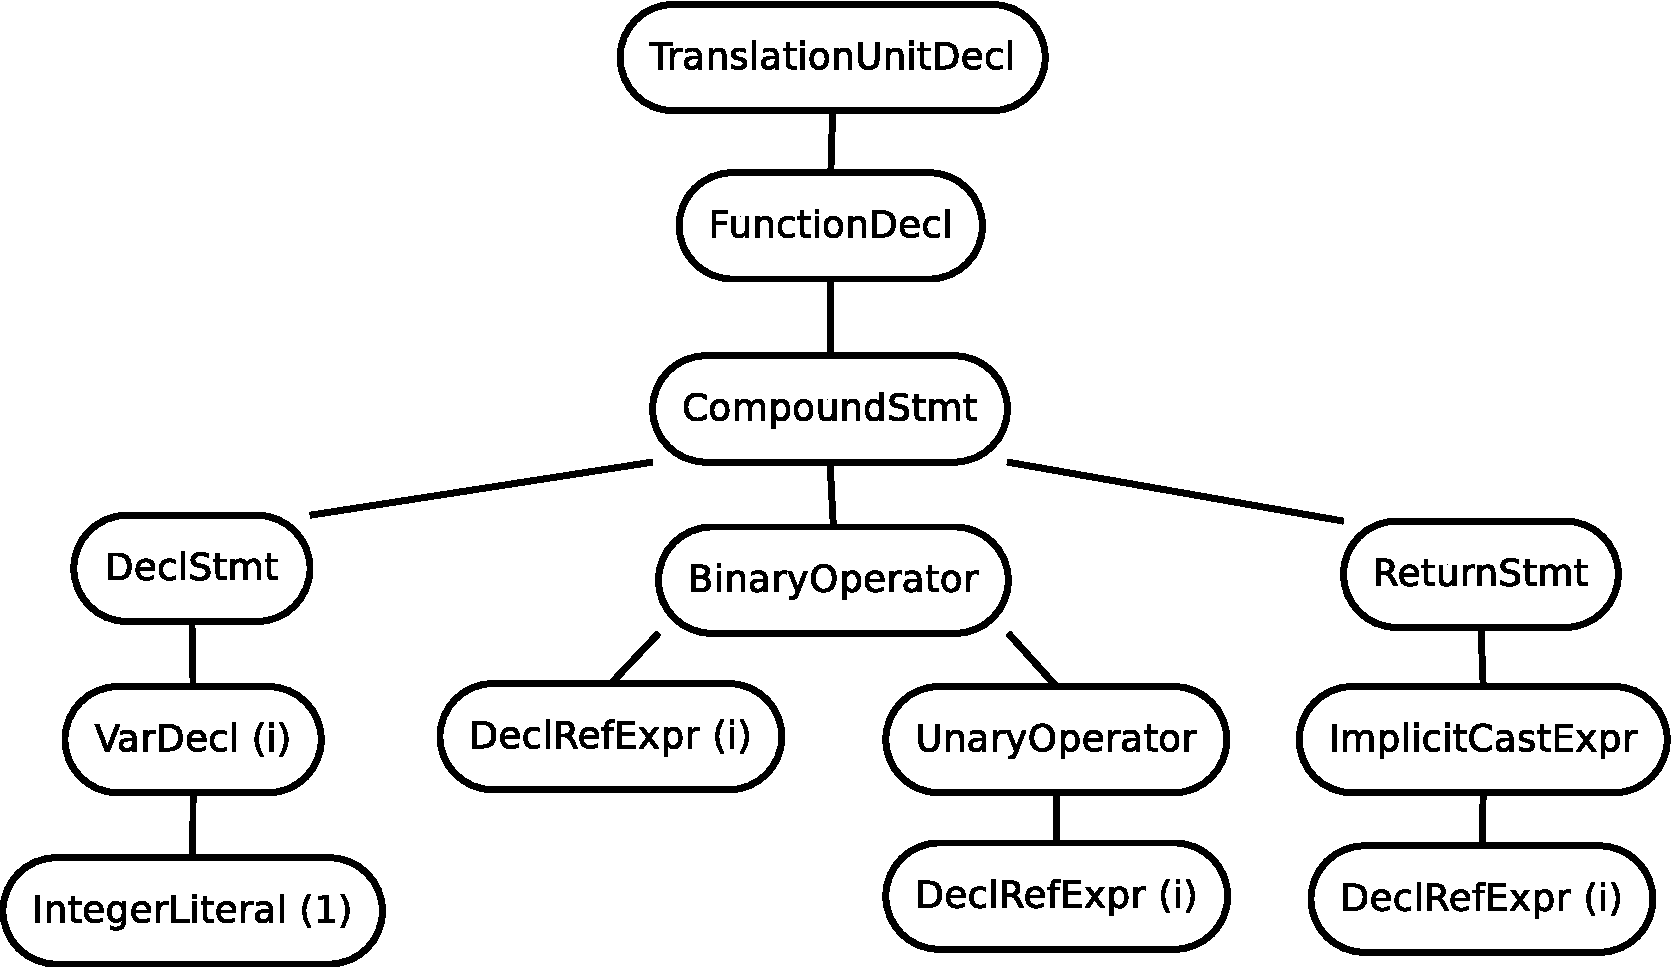
\includegraphics[width=1\textwidth]{fig/example1G.pdf}
\end{figure}

As we can see, we can, by definition of individual AST nodes, determine what (if any) child node is the side effect going to be applied to. Then when we go several levels up from node A towards the root and stop in node B, we can conclude that the whole subtree of B in which the node A is still has the side effect on the same memory address. We therefore can start from the DeclRefExpr nodes and while traversing the tree up to the root, decide whether the current node implies a side effect on a given DeclRefExpr.

%%%%%%%%%%%%
\section{L-value scope}
Some expressions keep an address of the given operand, meaning it can be used later in some parent node as an lvalue and, e.g., be assigned to. Consider this code:

\begin{lstlisting}
int main(void){
    int i = 2;
    int a = 3;
    *(a==3?&i:&i) = 42;
    return i;
}

\end{lstlisting}

In this example, it is the case of \verb|&i|. Some other expressions, however, get rid of the operand address irreversibly and we can be sure it will never be used as an L-value until its next occurence. An example of this is the \verb|b| variable in the conditional operator from the code above: it can never be used as an l-value in the whole subtree with the assignment it appears in as the conditional operator just uses it and throws it away.

%%%%%%%%%%%%
\section{Node tagging}
From this, we can conclude that every node can be tagged either as "implying a side effect", "not implying anything" or "making side effect impossible" on certain memory place given by certain DeclRefExpr. We can do this for each DeclRefExpr. The picture from the above would then be tagged as shown on figure \ref{ASTtagged}.
\begin{figure}
    \caption{Example 1~(\ref{example1}) AST graphical representation -- tagged}
    \label{ASTtagged}
    \centering
        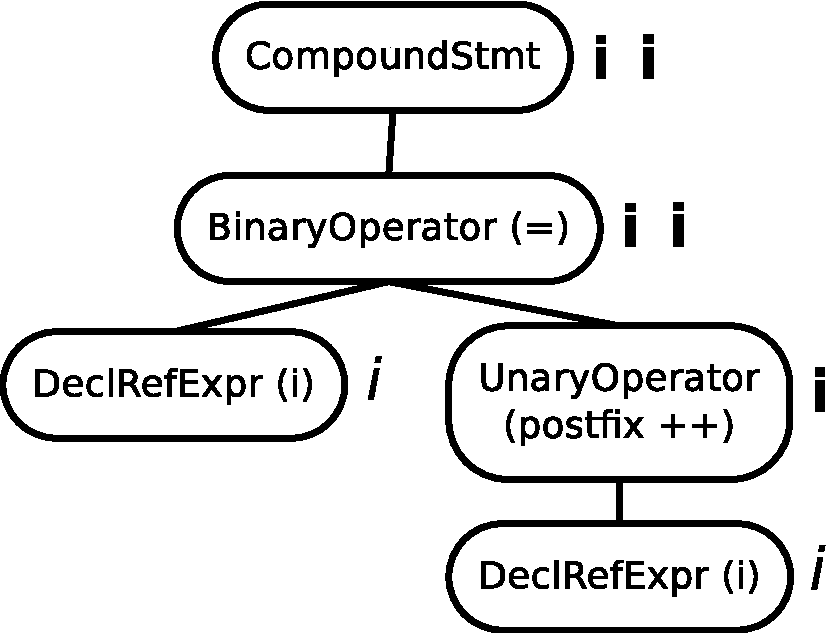
\includegraphics[width=0.6\textwidth]{fig/example1G-tagged.pdf}
\end{figure}

We began tagging from the left DeclRefExpr. It surely can be used as an l-value but the expression itself implies no side effect, hence the blue tag ("not implying anything"). We went towards the root and as we passed the \verb|BinaryExpression (=)|, we mark it as an expression implying a side effect on \verb|i| (red tag) as it modifies the memory contents of \verb|i|. We continued to the top implicitly marking all the parent nodes as having a side effect on \verb|i|. Then we can do the same for the right DeclRefExpr and as we see two red tags of the same variable, we can say we found an undefined behavior.

%%%%%%%%%%%%
\section{Aliasing}
So far, we can determine \verb|i = i++| leads certainly to undefined behavior, but we can not go so far in this simple case:

\begin{lstlisting}
int main(){
	int i = 0;
	int *j = &i;
	i = (*j)++;
    return i;
}
\end{lstlisting}

\verb|*j| may and may not alias with \verb|i|. After the tagging, I will therefore need to be able to determine whether two memory spaces alias.

This can not, however, be done in Clang on the AST level (as long as I am not willing to implement my own alias analysis, which would be useless). Neither is it possible to analyze AST using tools conventionally used for alias analysis. This said, the goal of the first part of my project is to merely generate a set of constraints saying under what conditions the undefined behavior may occur. For this example, the goal is to generate a rule saying "On the row 4, there is undefined behavior \emph{if} \verb|*j| aliases with \verb|i|". This can be checked later on either in LLVM or using some external alias analysis.

%%%%%%%%%%%%
\section{Functions}
I do not, however, know of any alias analysis capable of determining whether two objects in different functions alias.

\begin{lstlisting}
int f(int *a){
    (*a)++;
    return *a;
}

int g(int *b){
    (*b) *= 2;
    return *b;
}

int main(){
    int i = 1;
    i = f(&i) + g(&i);
    return i;
}
\end{lstlisting}

In this case, the most efficient and usable approach is probably just stating that if the function \emph{can} use its argument as an l-value (meaning it has the object pointer or some object it can get it from as an argument), I will assume it \emph{does}.

%%%%%%%%%%%%
\section{Output format}
For sake of portability, the output of the first (Clang) phase will not be forwarded directly to LLVM (which is probably the tool that will be used for alias analysis), but to the standard output instead. The output must contain the following information:

\begin{itemize}
\item Function in which the variables are to be checked for aliasing
\item Location of the statement with potentially undefined behavior
\item Variables to be checked; if they alias, undefined behavior occurs
\end{itemize}

\begin{lstlisting}
Possible undefined behavior in function "main" at [16,9] - "*j" aliases with "*k"
Possible undefined behavior in function "main" at [16,5] - "*j" aliases with "i"
Possible undefined behavior in function "main" at [16,5] - "*k" aliases with "i"
\end{lstlisting}

This output can then be used by any external alias analysis.

